\documentclass{beamer}
\usepackage{verbatim}
\usepackage[utf8]{inputenc}
\usetheme{Madrid}
\setlength{\parindent}{1cm} % padrão 15pt.
\setlength{\parskip}{1cm plus 4mm minus 3mm} %paragrafros
\usecolortheme{structure}

\title{Rendering e Projeção/Observação de cenas 3D}

\author[Igor, Lucas, Vinicius]
{
	Igor Jordany Richtic Silva\inst{1} 
	\and Lucas Afrânio Silva de Siqueira\inst{1} 
	\and Vinicius Antonio da Conceição\inst{1}
}

\institute[IC]
{
	\inst{1} Instituto de Computação\\ Universidade Federal de Mato Grosso
}

\date[2017]
{
	Agosto 2017
}

%\logo{
\includegraphics[height=1.5cm]{ufmtblue.jpg}}

\begin{document}
	%slide 1
	\begin{frame}
		\maketitle
	\end{frame}
	%slide 2
	\begin{frame}
		\frametitle{Roteiro}
		\begin{itemize}
		\item Rendering
		\begin{itemize}
			\item Fases do processo de Realismo Visual
			\item Realismo por passadas
			\item Rasterização
			\item Amostragem, Aliasing, e Anti-aliasing
			\item Superamostragem
			\item Exemplo de Anti-alising em linhas
			\item Remoção de elementos ocultos
			\item Z-Buffer
		\end{itemize}
		\item Projeção/Observação
		\begin{itemize}
			\item Projeção paralela
			\item Projeção perspectiva
			\item Leis da perspectiva
			\item Tipos de perspectivas
		\end{itemize}
		\item Dúvidas
		\end{itemize}
	\end{frame}
	%slide 3
	\begin{frame}
		\frametitle{Rendering}
		\begin{itemize}
		\item Podemos interpretar o processo de rendering como o de converter dados em uma imagem realística ou simplesmente sintetizar um objeto ou cena até ter-se deles uma aparência de algo real e não de formas inteiramente criadas no computador.\\
		\item Essa síntese de uma imagem (uma cena ou objeto) é criá-la em termos da definição dos dados dos objetos que a compõem. Isso se faz a partir da geometria da cena, das informações sobre os materiais de que são feitos os objetos (suas cores e texturas), das condições de iluminação ambiente e da posição de observação da cena.
		\end{itemize}
	\end{frame}
	%slide 4
	\begin{frame}
		\frametitle{Fases do processo de Realismo Visual}
		\begin{center}
			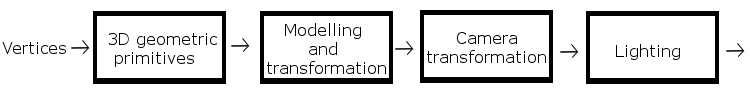
\includegraphics[height=1.5cm]{pipeline1.png}
		\end{center}
		\begin{center}
			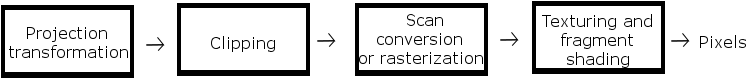
\includegraphics[height=1.2cm]{pipeline2.png}
		\end{center}
	\end{frame}
	%slide 5
	\begin{frame}
		\frametitle{Realismo por passadas}
		\begin{center}
			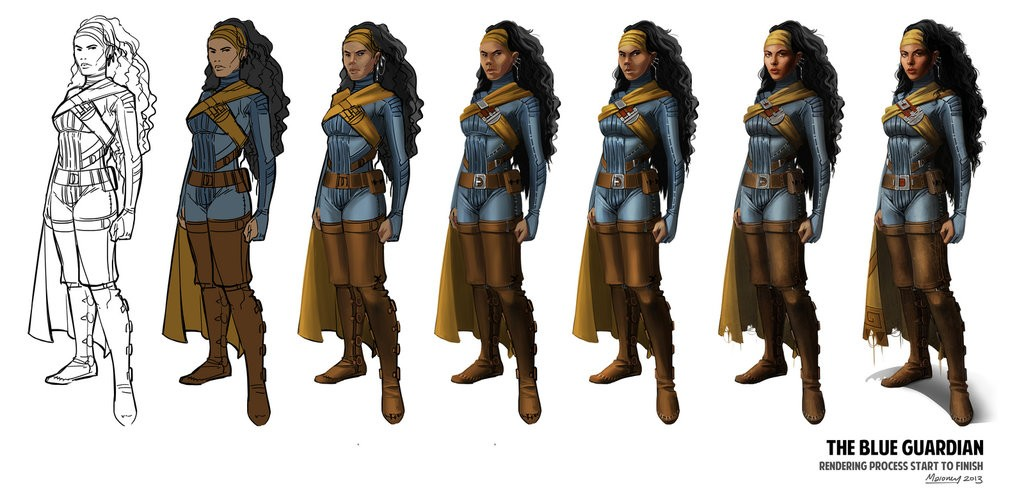
\includegraphics[height=6cm]{guarda.png}
		\end{center}
	\end{frame}
	%slide 6
	\begin{frame}
		\frametitle{Rasterização}
		\begin{itemize}
		\item Rasterização é um processo de amostragem
		\item Problemas de aliasing são esperados 
		\item Cada primitiva pode gerar um grande número de pixels 
		\item Em geral, rasterização é feita por hardware
		\begin{center}
			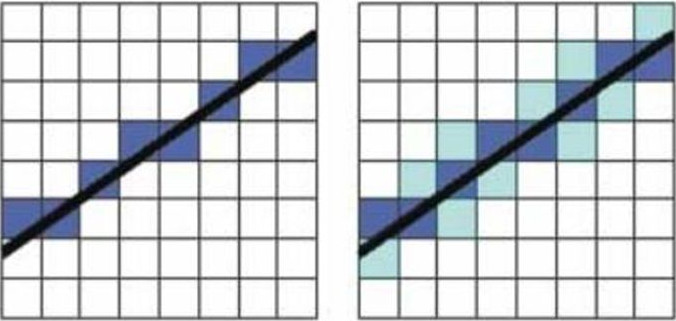
\includegraphics[height=4cm]{Rasterizacao.jpg}
		\end{center}
		\end{itemize}
	\end{frame}
	%slide 7
	\begin{frame}
		\frametitle{Amostragem, Aliasing, e Anti-aliasing}
		\begin{itemize}
		\item A linha, que no universo físico é contínua, é amostrada em uma matriz finita 2D de pixels.
		\item Tal discretização pode causar distorções visuais como cisalhamento ou efeito de escada. Essas distorções são chamadas de aliasing. Para reduzir o problema ,usa-se uma técnica chamada antialiasing.
		\item A técnica consiste em uma superamostragem (uma vez que o aliasing é causada por uma subamostragem).
		\begin{center}
			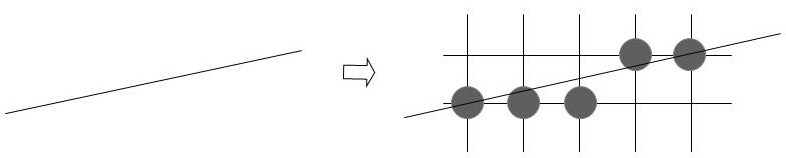
\includegraphics[height=2cm]{aliasing.jpg}
		\end{center}
		\end{itemize}
	\end{frame}
	%slide 8
	\begin{frame}
		\frametitle{Superamostragem}
		\begin{itemize}
		\item Superamostragem = Amostrar um objeto numa resolução maior do que será reconstruído.
		\begin{center}
			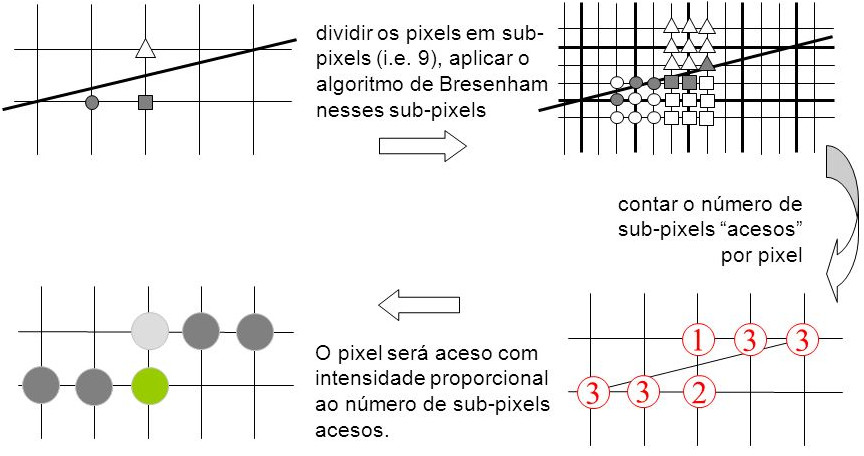
\includegraphics[height=6cm]{superamostragem.jpg}
		\end{center}
		\end{itemize}
	\end{frame}
	%slide 9
	\begin{frame}
		\frametitle{Exemplo de Anti-alising em linhas}
		\begin{itemize}
		\item Observe que quando a cor de fundo não é preto, o antialiasing deve fazer uma composição da intensidade com a cor de fundo.  
		\item Anti-aliasing é necessário não só para linhas, mas também para polígonos e texturas (o que já é mais complicado).
		\begin{center}
			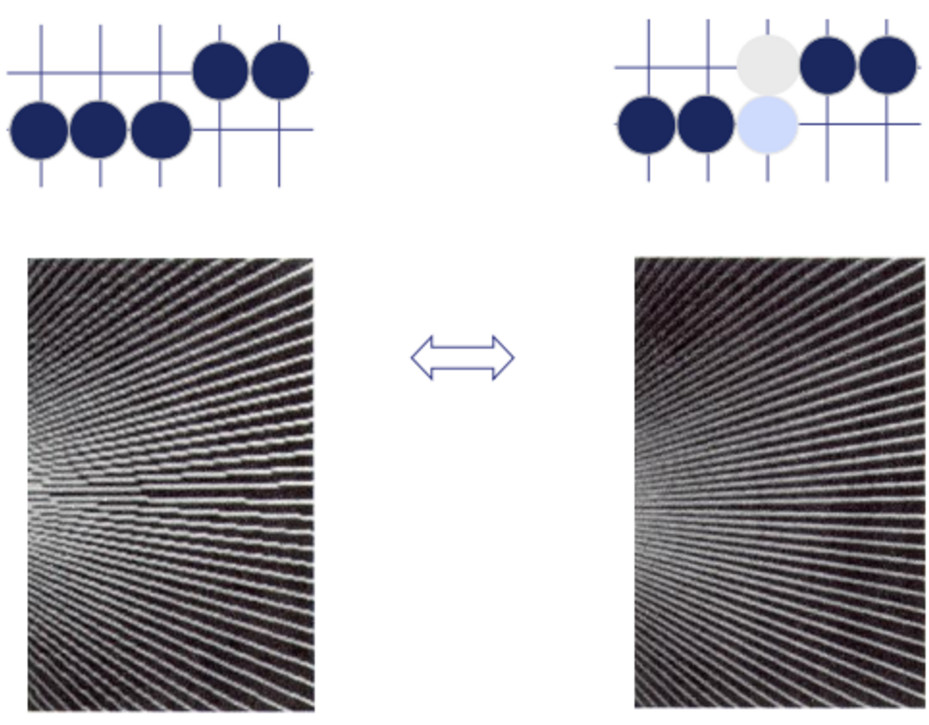
\includegraphics[height=6cm]{antaliasing.jpg}
		\end{center}
		\end{itemize}
	\end{frame}
	%slide 10
	\begin{frame}
		\frametitle{Remoção de elementos ocultos}
		\begin{center}
			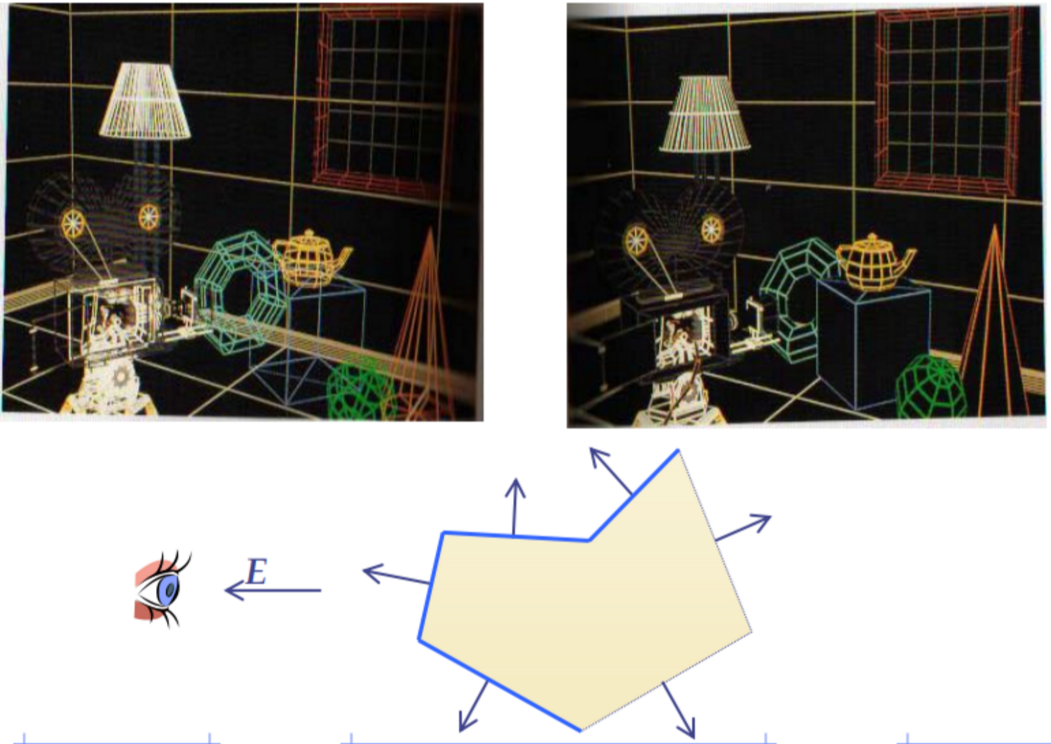
\includegraphics[height=8cm]{remocao.png}
		\end{center}
	\end{frame}
	%slide 11
	\begin{frame}
		\frametitle{Z-Buffer}
		\begin{itemize}
		\item Buffers são áreas reservadas de memória utilizadas para determinados propósitos. 
		\item Em aplicações de animação, por exemplo, o double-buffer permite que as sucessivas renderizações sejam feitas de modo suave, sem o efeito indesejável de piscar entre cada atualização da janela de visualização. 
	 	\item O z-buffer é bastante comum em aplicações gráficas e é utilizado para calcular a distância do observador e remover superfícies ou partes ocultas de objetos sobrepostos.\\
		glutInitDisplayMode(GLUT\_DOUBLE\textbar GLUT\_RGB\textbar GLUT\_DEPTH)
		\end{itemize}
	\end{frame}
	%slide 12
	\begin{frame}
		\frametitle{Projeção}
		\begin{itemize}
		\item No mundo real temos um objeto ex: uma torre. A torre está em um plano 3D. Você pode mover se ao redor da torre sobre o solo ou sobre o ar, e tirar uma fotografia que será convertida para uma imagem 2D.\\
		Dependendo de onde estiver a câmera você verá uma diferença na imagem, como sobras, nível de luz etc..
		\end{itemize}
	\end{frame}
	%slide 13
	\begin{frame}
		\frametitle{Projeção}
		\begin{center}
			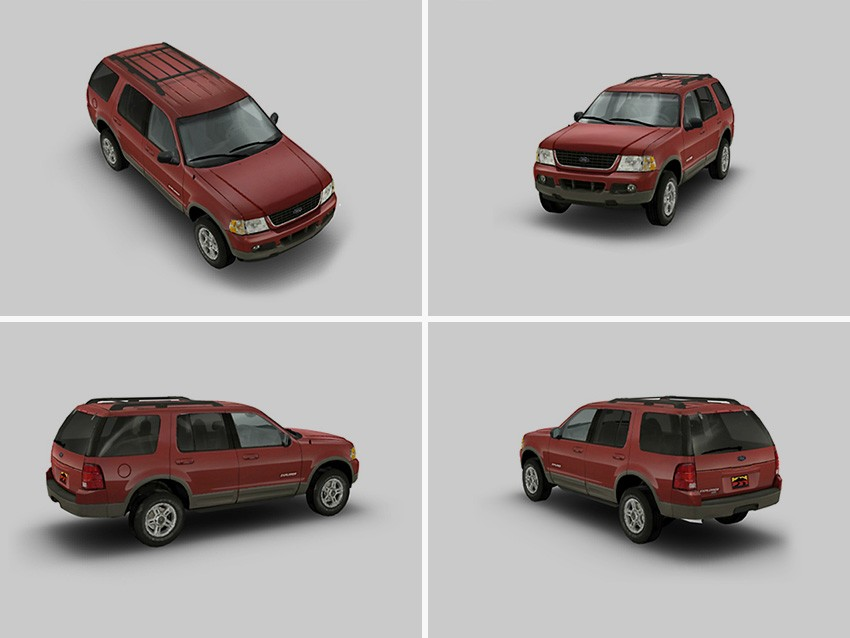
\includegraphics[height=8cm]{carros.png}
		\end{center}
	\end{frame}
	%slide 14
	\begin{frame}
		\frametitle{Projeção}
		\begin{itemize}
		\item No computador temos que simular um ponto de visão e a partir dele gerar nossos cenários.
		\end{itemize}
		\begin{center}
			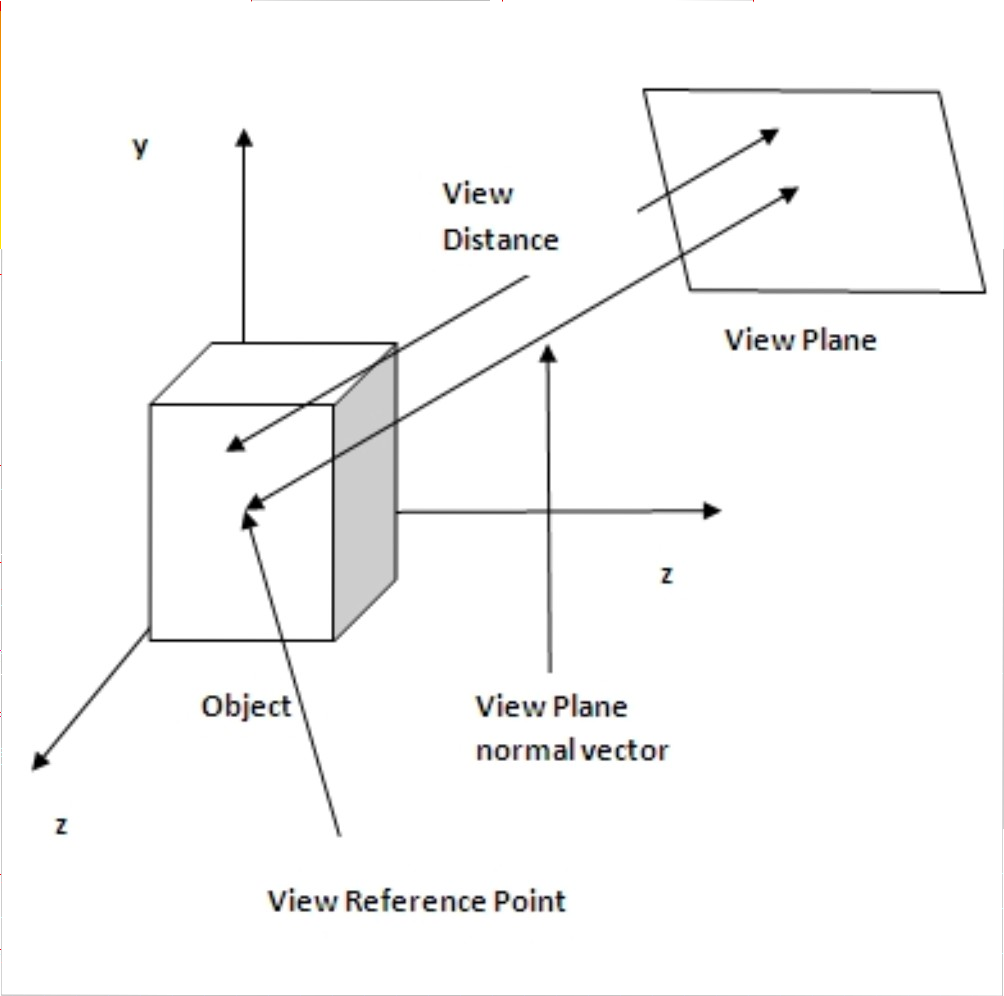
\includegraphics[height=6cm]{pontodevisao.png}
		\end{center}
	\end{frame}
	%slide 15
	\begin{frame}
		\frametitle{Projeção}
		Os tipos de projeções dependem de 2 fatores:
		\begin{itemize}
		\item Posição do observador
		\item Localização e orientação do plano de projeção
		\end{itemize}
		\begin{center}
			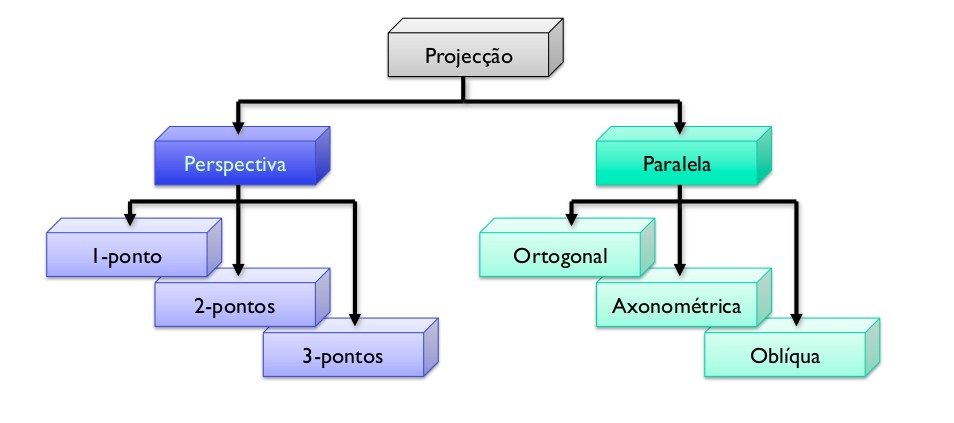
\includegraphics[height=5cm]{fluxoproj.png}
		\end{center}
	\end{frame}
	%slide 16
	\begin{frame}
		\frametitle{Projeção paralela}
		\begin{itemize}
		\item Se o objeto está alinhado com os eixos, o resultado é uma projeção ortogonal.\\
		Caso contrário, é uma projeção axonométrica.
		\item Se o plano de projeção intersecta os eixos XYZ à mesma distância relativamente à origem, o resultado é
uma projeção isométrica.
		\end{itemize}
	\end{frame}
	%slide 17
	\begin{frame}
		\frametitle{Projeção paralela}
		\begin{center}
			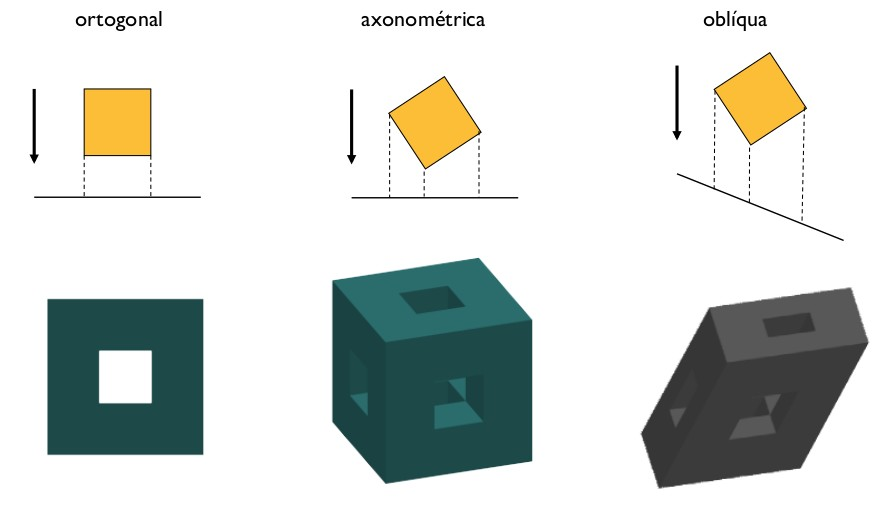
\includegraphics[height=5.5cm]{ortogonal.png}
		\end{center}
	\end{frame}
	%slide 18
	\begin{frame}
		\frametitle{Projeção perspectiva}
		\begin{itemize}
		\item O observador está a uma distância finita do/a objeto/cena. pontos (observadores).
		\item As projetantes não são paralelas e convergem para um ou mais.
		\end{itemize}
	\end{frame}
	%slide 19
	\begin{frame}
		\frametitle{Projeção perspectiva}
		\begin{center}
			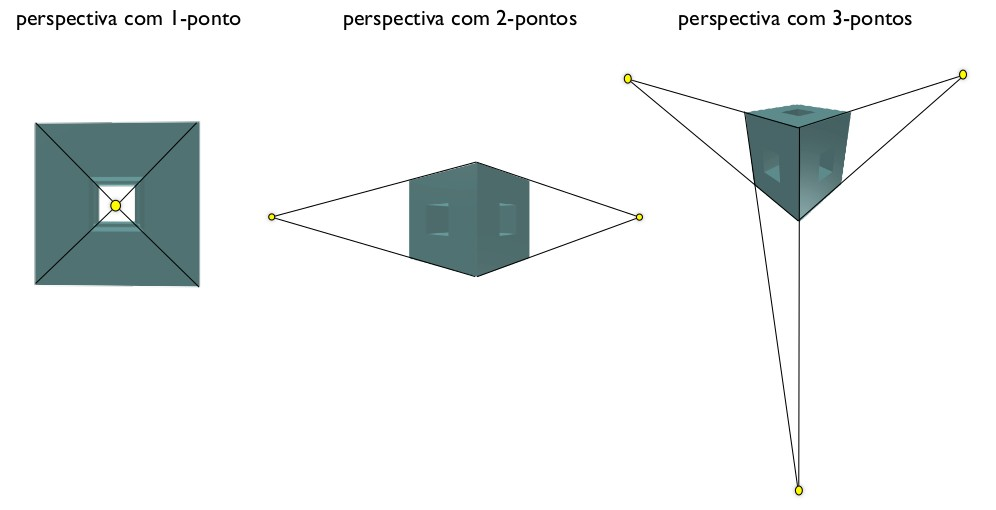
\includegraphics[height=6cm]{perspectiva.png}
		\end{center}
	\end{frame}
	%slide 20
	\begin{frame}
		\frametitle{Leis da perspectiva}
		\begin{itemize}
		\item Tudo parece diminuir à medida que se afasta do observador (desenhista).
		\end{itemize}
		\begin{center}
			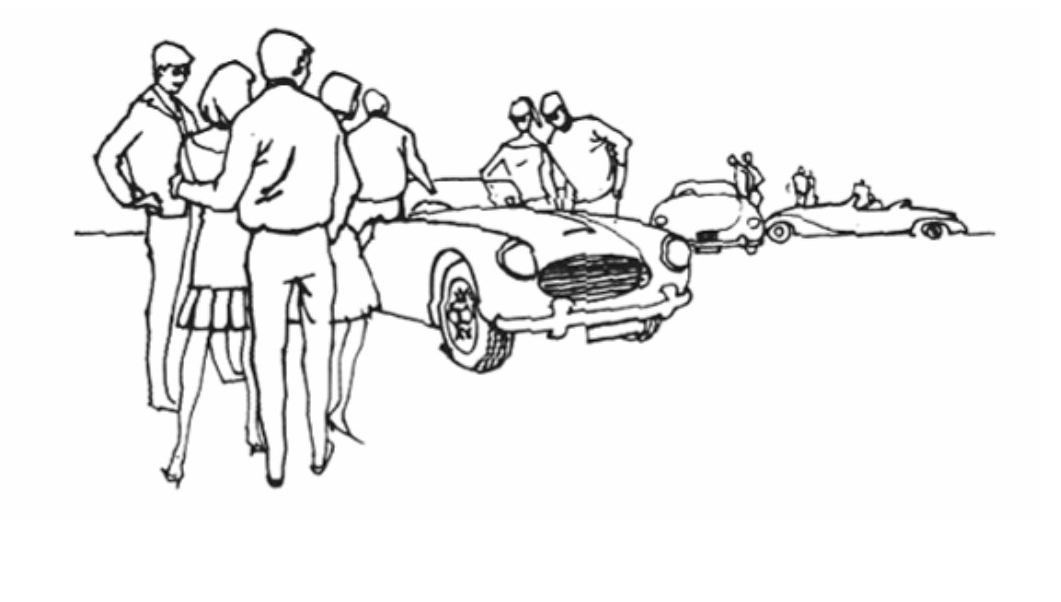
\includegraphics[height=5.5cm]{foto.jpg}
		\end{center}
	\end{frame}
	%slide 21
	\begin{frame}
		\frametitle{Leis da perspectiva}
		\begin{itemize}
		\item Linhas retas horizontais ou verticais tendem a se apresentar diagonais quando “entram” para o fundo.
		\item Já quando “estão” à sua frente, mantém sua perpendicularidade.
		\end{itemize}
		\begin{center}
			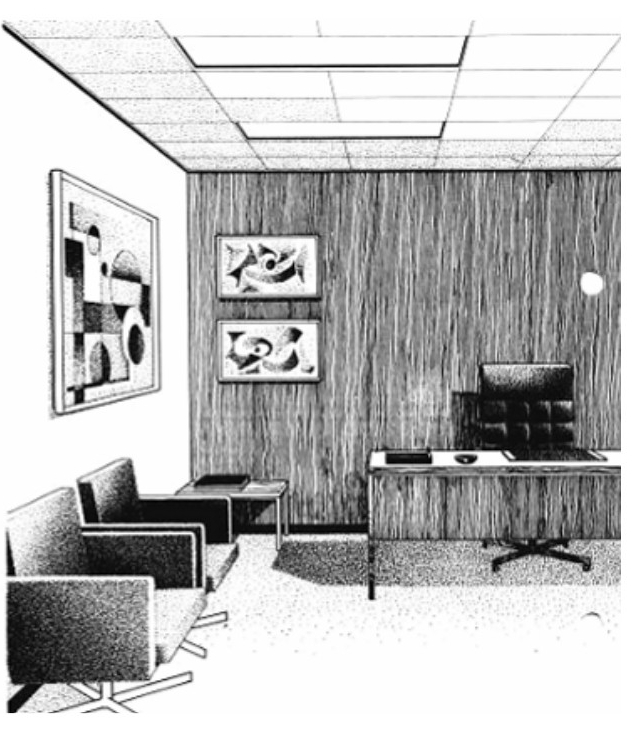
\includegraphics[height=5.5cm]{foto2.jpg}
		\end{center}
	\end{frame}
	%slide 22
	\begin{frame}
		\frametitle{Tipos de Perspectivas}
		\begin{center}
			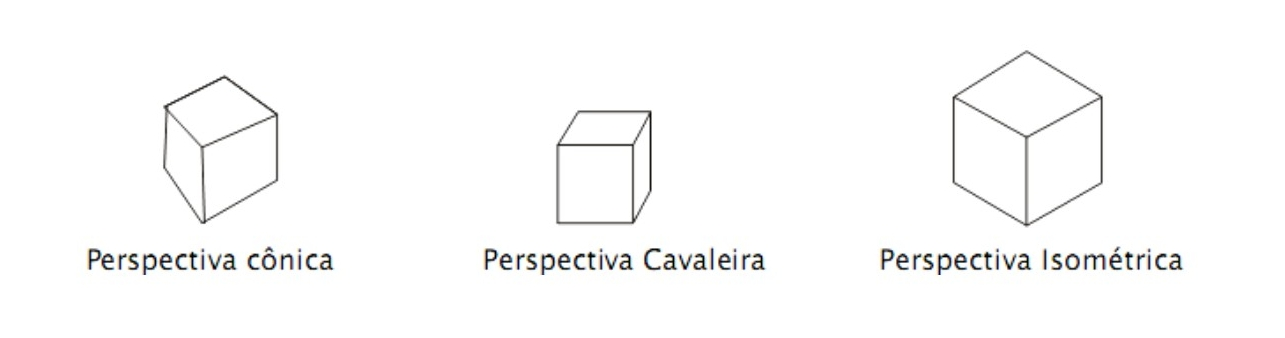
\includegraphics[height=3.3cm]{foto3.jpg}
		\end{center}
		\begin{itemize}
		\item Cada tipo de perspectiva mostra o objeto de um jeito.
		\item Comparando as três formas de representação, nota-se que a perspectiva isométrica é a perspectiva que dá a sensação de menor deformação do objeto.
		\end{itemize}
	\end{frame}
	%slide 23
	\begin{frame}
		\frametitle{Dúvidas?}
		\begin{center}
			
\includegraphics[height=6cm]{mario.png}
		\end{center}
	\end{frame}
\end{document}